\documentclass{article}

\usepackage[spanish]{babel}

\usepackage[letterpaper,top=2cm,bottom=2cm,left=3cm,right=3cm,marginparwidth=1.75cm]{geometry}

\usepackage{amsmath}
\usepackage{graphicx}
\usepackage{enumitem}
\usepackage{comment}
\usepackage{wrapfig}
\usepackage[colorlinks=true, allcolors=blue]{hyperref}

\title{Redes Tema 5. Capa de enlace}
\author{Martín González Dios 
\href{https://github.com/martindios}{\includegraphics[height=0.5cm]{github.png}}}

\begin{document}
\maketitle

\textbf{Transmite bloques de bits de un lado al otro de un enlace punto a punto }(emisor y receptor en los extremos) o \textbf{determina el acceso al medio en redes de difusión} (medio de transmisión compartido por varios emisores). La unidad de datos del protocolo (PDU) es la trama o el marco y la capa de enlace añade una cabecera ETH. 

\textbf{Los hosts (origen/destino) y routers son los nodos, y los LANs o redes punto a punto, los enlaces}. La capa de enlace se implementa en la tarjeta de red (adaptador) y el adaptador se conecta al nodo. Los protocolos de la capa de enlace definen el formato de las tramas y las acciones de los nodos cuando envían o reciben tramas. \\


\begin{wrapfigure}[]{r}{0.45\linewidth}
    \centering
    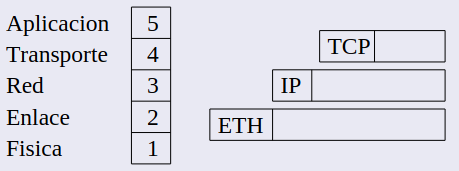
\includegraphics[width=0.8\linewidth]{img-t5/img_972_54.png}
    \caption{Cabeceras en las distintas capas}
\end{wrapfigure}

La capa de enlace \textbf{proporciona servicios a nivel de red} en el ámbito nodo a nodo como el
\textbf{encapsulado/desencapsulado de datagramas}. Otros servicios posibles son el \textbf{entramado o delimitado de tramas}, el acceso al enlace con el protocolo MAC (control de acceso al medio), la entrega fiable (confirmaciones y retransmisiones), el control de flujo, la detección (sofisticada) y corrección (paridad, checksum, CRC) de errores o el half/full-duplex (transmisión en uno o ambos sentidos). La capa de enlace añade su propia cabecera.

\section{Modelo IEEE 802}

\begin{wrapfigure}[]{r}{0.45\linewidth}
    \centering
    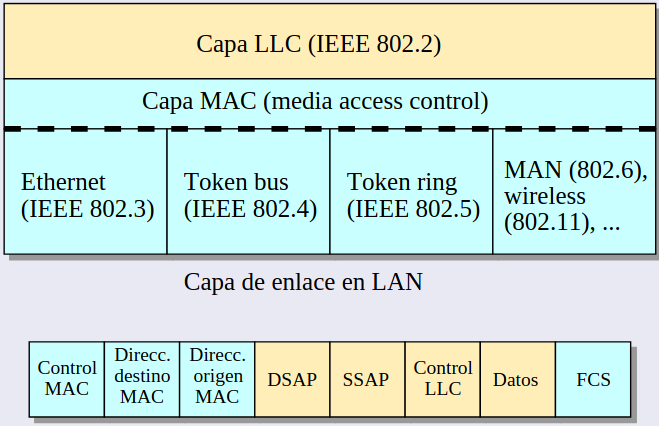
\includegraphics[width=\linewidth]{img-t5/img_682_18.png}
    \caption{Formato de trama}
\end{wrapfigure}

\textbf{Define los principales tipos de LANs} (Red de Área Local) y establece un \textbf{modelo para la capa de enlace en LANs} (LANs de difusión). La capa de enlace está \textbf{dividida en 2 subcapas} ya que la lógica necesaria para gestionar el acceso a un medio compartido no está en la capa de enlace de datos tradicional.

\begin{itemize}
    \item \textbf{Capa de enlace lógico (LLC)}: es una interfaz con las capas superiores que incluye control de errores y de flujo. El tipo de servicio puede ser sin conexión ni confirmaciones (control capas superiores), sin conexión con confirmaciones, o con conexión y confirmaciones.

    \item \textbf{Capa de acceso al medio (MAC)}: ensambla y desensambla datos en tramas con campos dirección y detección de errores.
\end{itemize}
(Para un mismo LLC hay disponibles varios MAC)

\newpage

\section{Direcciones MAC}

\begin{wrapfigure}[]{r}{0.58\linewidth}
    \centering
    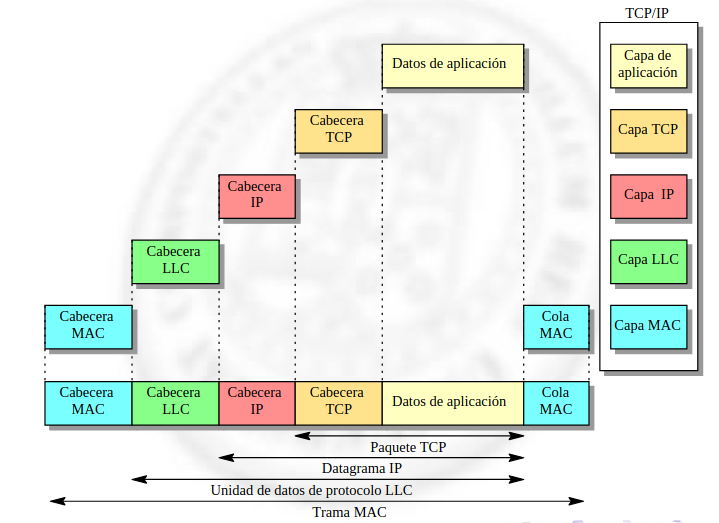
\includegraphics[width=\linewidth]{img-t5/img_137_27.png}
    \caption{Protocolos LAN}
\end{wrapfigure}

En \textbf{TCP/IP hay 2 direcciones}. La dirección \textbf{MAC} en el enlace o LAN (la usan los adaptadores), y fuera, en Internet, se eliminan las cabeceras MAC y se usan las \textbf{direcciones IP}. 

En Ethernet \textbf{todos los nodos tienen una dirección única} (dir. MAC de 6 bytes) proporcionada por el adaptador Ethernet y fijada en una memoria ROM. 
Hay \textbf{2 direcciones Ethernet especiales}, la \textbf{broadcast} (todos los bits a 1) que envía a todos los nodos de la red, y la \textbf{multicast} (bit menos significativo del 1er byte a 1) que envía a un grupo de nodos de la red. 

Un nodo acepta tramas unicast, multicast, broadcast y cualquier valor si está en \textbf{modo promiscuo}. 
Las tarjetas de red usan direcciones MAC, pero los nodos usan IPs. Para esto el \textbf{protocolo ARP} tiene una \textbf{tabla (caché ARP)} con \textbf{correspondencias IP-MAC}. Cuando ARP recibe una IP devuelve la MAC si está en la tabla o emite una trama broadcast con la IP para que el adaptador de esa IP responda con su MAC, almacenándola en la caché ARP y devolviéndosela al que la pidió (Las entradas de la caché ARP se eliminan a los 15 mins).

\begin{figure}[h]
    \centering
    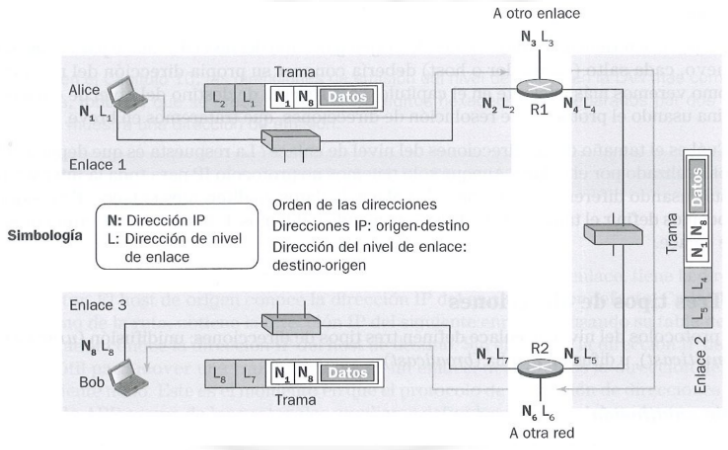
\includegraphics[width=0.75\textwidth]{img-t5/img_071_39.png}
    \caption{Direcciones en la capa de enlace}
\end{figure}

\newpage

\section{Ethernet}

La red Ethernet es el \textbf{tipo de LAN más sencillo y común}. Es un servicio no fiable con red de difusión. Funciona sobre cable coaxial (topología bus), par trenzado (topología estrella) y fibra óptica, a muchas velocidades distintas. \\

\begin{wrapfigure}[]{r}{0.5\linewidth}
    \centering
    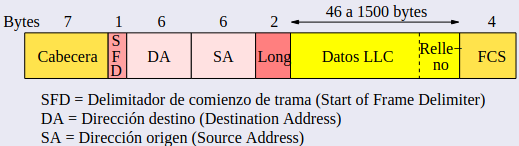
\includegraphics[width=\linewidth]{img-t5/img_324_16.png}
    \caption{Formato de trama MAC Ethernet}
\end{wrapfigure}

La \textbf{trama MAC Ethernet} tiene una cabecera de 7 bytes para sincronización, un byte SDF que
indica el comienzo de la trama, 2 bytes para la longitud de los datos o para indicar el protocolo
de red (Ethernet DIX), un campo relleno (traza entre 64 y 1518 bytes) y un campo FSC (Frame
Check Sequence) de 4 bytes. \\


Ethernet es una \textbf{red de difusión que usa el protocolo MAC} para decidir quién transmite. Usa \textbf{CSMA/CD} (acceso múltiple por detección de portadora con detección de colisión), un \textbf{algoritmo de acceso al medio compartido}. Para recibir todos los adaptadores escuchan continuamente y para
transmitir el adaptador escucha el medio, esperando a que el cable quede libre (+ intervalo de seguridad) si está ocupado o transmitiendo si está libre. Se pueden producir colisiones (2 señales en el medio a la vez). Cuando un nodo detecta una acaba de \textbf{transmitir la cabecera de la trama, emite una secuencia de 32 bits} (jamming sequence), detiene la transmisión y usa el algoritmo de espera exponencial binaria (exponential backoff). \\ 

Para detectarlas \textbf{el emisor escucha el cable mientras transmite}. El tiempo entre que un nodo ocupa el medio y la transmisión alcanza los otros se llama \textbf{tiempo de vulnerabilidad}. Durante este tiempo el resto de nodos ven el medio libre, y si transmitiesen alterarían los datos del medio. Por esto se establece $t_{trama}$ > 2$t_{prop}$ (tamaño de trama mínimo o longitud de enlace máximo). \\

El algoritmo de (\textbf{espera exponencial binaria}) divide el tiempo en ranutas de T = 2$t_{prop\_max}$. Las estaciones esperan 0 o T para retransmitir. Si hay colisión se espera aleatoriamente 0T...3T. Si hay otra espera entre 0T y ($2^n$ - 1)T. Desde 10 colisiones elige entre 0T y 1023T. Tras 16 desiste, informa y delega en capas superiores. \\

\newpage

\begin{wrapfigure}[]{r}{0.35\linewidth}
    \centering
    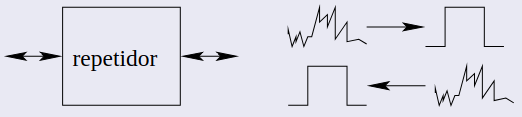
\includegraphics[width=\linewidth]{img-t5/img_050_02.png}
    \caption{Funcionamiento del repetidor}
\end{wrapfigure}

Un \textbf{repetidor} es un dispositivo de capa física que trabaja sobre bits individuales. Copia bits que llegan por una interfaz en el resto de interfaces reconstruyendo el pulso de tensión. Tiene 2 o más interfaces y se usa en transmisiones de distancias largas. \\

\textbf{Hub o concentradores} (obsoletos): dispositivo de capa física que trabaja sobre bits individuales. Regenera un bit y lo envía por todas las interfaces. Si llegan a la vez por distintos interfaces, el hub informa a los adaptadores de que hubo colisión.

\begin{figure}[h]
    \centering
    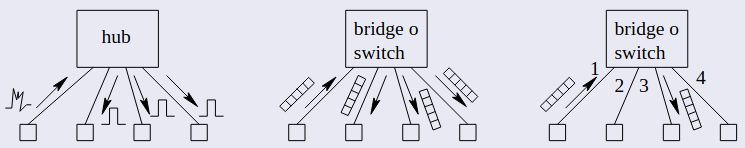
\includegraphics[width=0.55\textwidth]{img-t5/img_117_05.png}
    \caption{Funcionamiento del hub}
\end{figure}



\textbf{Topologías de Ethernet}:
\begin{itemize}
    \item \textbf{Topología bus} (obsoleta): bus de cable coaxial usando conectores T con terminadores en los extremos. Permite hasta 4 repetidores y en cada segmento se limitan los adaptadores. Nomenclatura: $<$Mbps$>$$<$transmisión$>$$<$centenas m$>$ Ejemplo: 10base5 $\xrightarrow{}$ 10 Mbps, banda de base y segmento de 200m.
    \begin{figure}[h]
    \centering
    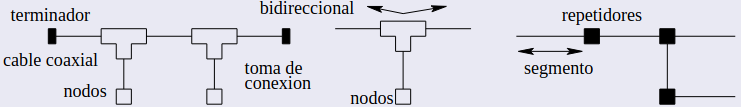
\includegraphics[width=0.65\textwidth]{img-t5/img_377_16.png}
    \caption{Topología bus}
    \end{figure}

    \item \textbf{Topología estrella}: hub o conmutador en el centro con par trenzado o fibra óptica. Cada nodo tiene un par trenzado o fibra óptica de entrada y otro de salida. La distancia está limitada y el funcionamiento del protocolo es equivalente al de bus. Nomenclatura: T par trenzado y F, S, L y E fibra óptica. Ejemplo: 100base-TX (Fast Ethernet de par trenzado): 100 Mbps, banda de base y longitud de 100 m.
    
\end{itemize}

Los \textbf{puentes (bridges)} y \textbf{conmutadores (switches)} son dispositivos de capa de enlace que trabajan a nivel de tramas Ethernet procesando sus campos. Disponen de
colas en las interfaces de salida (los switches han dejado obsoletos a los puentes por tener más interfaces). \textbf{Aprenden la localización de los adaptadores}, guardando entradas para algunos en una tabla de reenvío (se borran tras varios minutos). Para guardar los adaptadores usan difusión y examinan las tramas que llegan (interfaz llegada $\xrightarrow{}$ localización adaptador / dirección origen $\xrightarrow{}$ identidad adaptador). \textbf{Si el adaptador destino está en la tabla, reenvía la trama solo por esa interfaz}, evitando colisiones ya que el resto no ven esa transmisión (aisla el tráfico). Si la interfaz origen coincide con el destino, descarta la trama (filtrado). Si las interfaces origen y destino son distintas puede haber transmisiones simultáneas
(más interfaces $\xrightarrow{}$ mayor tasa de transmisión elevada $\xrightarrow{}$ más transmisiones simultáneas).

\begin{figure}[h]
    \centering
    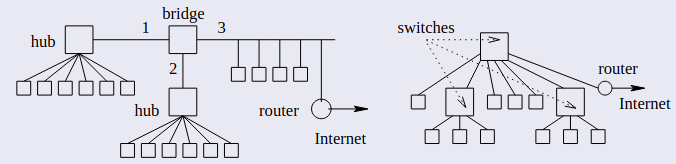
\includegraphics[width=0.65\textwidth]{img-t5/img_458_29.png}
    \caption{Puentes y conmutadores}
\end{figure}

\newpage

Tanto los \textbf{conmutadores} como los \textbf{routers} son dispositivos de almacenamiento y envío, pero \textbf{los primeros trabajan con cabeceras Ethernet} (capa enlace), mantienen tablas de conmutación, e implementan filtrado y algoritmos de aprendizaje mientras \textbf{los segundos trabajan con cabeceras IP} (capa red), mantienen tablas de rutas e implementan algoritmos de encaminamiento. \\
En muchos casos nos interesa usar \textbf{VLANs} (\textbf{redes de área local virtuales}). Los conmutadores compatibles con VLANs \textbf{nos permiten definir múltiples LANs virtuales} sobre una única red física. En VLANs basadas en puertos, los puertos del conmutador se dividen en grupos, siendo cada grupo una VLAN. Una tabla guarda que puertos pertenecen a cada grupo, y solo se mandan tramas dentro del grupo (aislamiento). De esta forma cualquier cambio implica solo reconfiguración de software.

\section{Conmutación de etiquetas multiprotocolo (MPLS)}
\textbf{Usa redes de circuitos virtuales para interconectar dispositivos IP}. Está entre la capa de red y la de enlace. Etiqueta datagramas permitiendo a los routers reenviarlos en base a etiquetas de longitud fija (mezcla cv y datagramas). Usa el direccionamiento y encaminamiento IP. \\
\textbf{Los routers de conmutación de etiquetas son compatibles con MPLS}. Reenvían tramas buscando etiquetas MPLS en su tabla sin necesitar IP destino.

\begin{figure}[h]
    \centering
    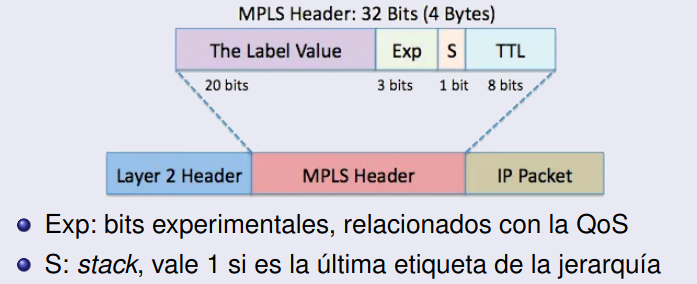
\includegraphics[width=0.65\textwidth]{img-t5/img_176_10.png}
    \caption{Cabeceras MPLS (RFC 3032)}
\end{figure}

\newpage

\section{Redes inalámbricas (WLAN)}
\begin{itemize}
    \item Redes simples (ad-hoc): \textbf{conexiones de igual a igual}, comunica 2 estaciones siempre que estén dentro del radio de alcance.
    
    \item Redes distribuidas (managed): tiene \textbf{una LAN troncal cableada} (distribution system) \textbf{que conecta los servidores y los puntos de acceso} (access points, AP). Cada AP da servicio a varias estaciones móviles, distribuyendo el espacio en celdas.
        \begin{figure}[h]
        \centering
        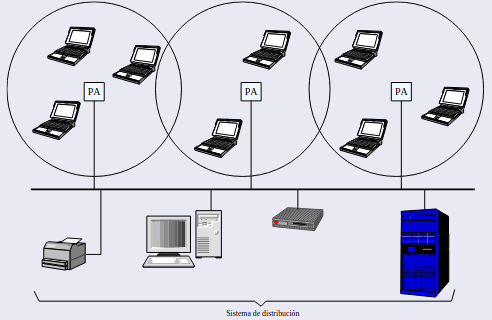
\includegraphics[width=0.45\textwidth]{img-t5/img_436_39.png}
        \caption{Redes distribuidas}
        \end{figure}    
\end{itemize}

Existe un protocolo \textbf{CSMA/CA} (o \textbf{MACA}, Multiple Access with Collision Avoidance) de acceso al medio. Cuando un host quiere transmitir sondea el medio, si está libre espera un intervalo grande (DIFS, Distributed Inter Frame Space) y transmite, si está ocupado escucha hasta que quede libre (y vuelve a esperar el DIFS). Si no queda libre usa la espera exponencial binaria. \\
\textbf{No tiene detección de colisiones}, los \textbf{hosts esperan los ACKs} y los \textbf{receptores esperan un intervalo corto} (SIFS) entre la recepción y el envío del ACK. \textbf{Para asegurar la transmisión usa tramas de control}: \textbf{RTS} (trama de petición de envío) y \textbf{CTS} (trama de reserva de canal). En una trama RTS se incluye el tiempo de ocupación, con lo que el resto de estaciones crean un temporizador NAV durante el cual no comprueban la actividad del canal. Dos estaciones pueden enviar RTS a la vez, pero \textbf{si el emisor no recibe un CTS asume colisión}.

\begin{figure}[h]
    \centering
    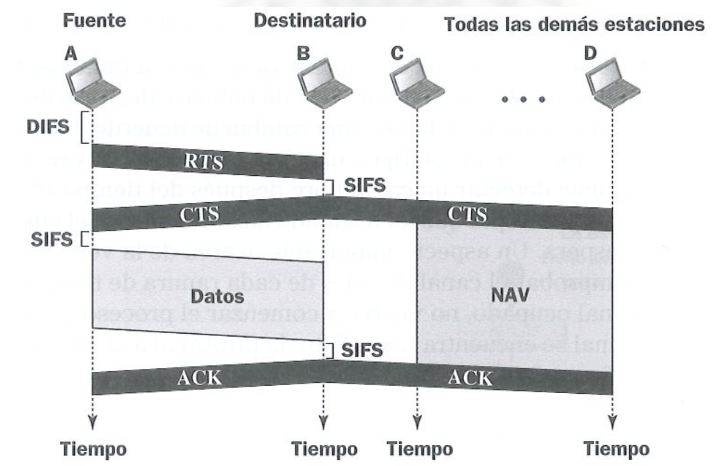
\includegraphics[width=0.65\textwidth]{img-t5/img_369_04.png}
    \caption{Protocolo de acceso al medio: CSMA/CA}
\end{figure}

\end{document}
